\documentclass[a4paper]{article}
\usepackage[fontsize=13pt]{scrextend}
\usepackage[utf8]{vietnam}
\usepackage{amsmath}
\usepackage{amsfonts}
\usepackage{xcolor}
\usepackage{titlesec}
\usepackage{mdframed}
\usepackage{amssymb}
\usepackage{pgf,tikz,pgfplots}
\usepackage{graphicx}
\graphicspath{ {../figures/} }
\usepackage{array}
\usepackage{cases}
\usepackage{listings}
\usepackage{tabulary}
\usepackage{color}
\usepackage{float} 
\usepackage{hyperref}
\usepackage{multirow}
\usepackage{booktabs, makecell}
\usepackage{eurosym}
\usepackage{siunitx}
\usepackage{minitoc}
\pgfplotsset{compat=1.5}
\usepackage{mathrsfs}
\usetikzlibrary{arrows, calc}
\usepackage{fancyhdr}
\pagestyle{fancy}
\pagestyle{empty}
\definecolor{dkgreen}{rgb}{0,0.6,0}
\definecolor{gray}{rgb}{0.5,0.5,0.5}
\definecolor{mauve}{rgb}{0.58,0,0.82}
\usepackage[
    backend=biber,
    style=numeric,
    natbib=true,
    url=true, 
    doi=true,
    eprint=false,
    sorting=nyt
]{biblatex}
\addbibresource{refs.bib}
\lstset{frame=tb,
  language=C++,
  aboveskip=3mm,
  belowskip=3mm,
  showstringspaces=false,
  columns=flexible,
  basicstyle={\small\ttfamily},
  numbers=none,
  numberstyle=\tiny\color{gray},
  keywordstyle=\color{blue},
  commentstyle=\color{dkgreen},
  stringstyle=\color{mauve},
  breaklines=true,
  breakatwhitespace=true,
  tabsize=3
}
\renewcommand{\listfigurename}{Danh sách hình}
\renewcommand{\listtablename}{Danh sách bảng}
\newcommand{\tabitem}{~~\llap{\textbullet}~~}
\usepackage[left=2cm,right=2cm,top=2cm,bottom=2cm]{geometry}
\author{Nguyễn Văn Lộc}
\newmdenv[linecolor=black,skipabove=\topsep,skipbelow=\topsep,
leftmargin=-5pt,rightmargin=-5pt,
innerleftmargin=5pt,innerrightmargin=5pt]{mybox}
\begin{document}
\fancyhf{}
\lhead{Báo cáo đồ án môn học Mạng máy tính}
\chead{}
\rhead{Địa điểm yêu thích}
\cfoot{\thepage}
\rfoot{}
\lfoot{}
\pagestyle{fancy}
\renewcommand{\headrulewidth}{0pt}
\renewcommand{\footrulewidth}{0pt}
\tableofcontents
\listoffigures
\listoftables
\begin{titlepage}
\begin{mybox}
\begin{center}
\fontsize{12}{12}\selectfont
\textbf{ĐẠI HỌC QUỐC GIA THÀNH PHỐ HỒ CHÍ MINH}\\
\textbf{TRƯỜNG ĐẠI HỌC KHOA HỌC TỰ NHIÊN}\\
\textbf{KHOA CÔNG NGHỆ THÔNG TIN}
\end{center}
\vskip 1 cm
\begin{figure}[H]
\begin{center}

\includegraphics[scale=0.25]{figures/logo}
\end{center}
\end{figure}
\vskip 1 cm
\begin{center}
\fontsize{18}{14}\selectfont
\textbf{SƯU LIỆU ĐỒ ÁN MÔN HỌC}\\
\fontsize{26}{16}\selectfont
\textbf{MẠNG MÁY TÍNH}\\
\fontsize{18}{12}\selectfont
\textbf{ĐỀ TÀI: Điều khiển máy tính thông qua email}
\end{center}
\vskip 1 cm
\fontsize{14}{12}\selectfont
\textbf{Giảng viên lý thuyết:} Thầy Đỗ Hoàng Cường\\
\textbf{Lớp:} 20TN\\
\textbf{Thành viên thực hiện:}
\begin{itemize}
\item 20120131 $-$ Nguyễn Văn Lộc
\item 20120536 $-$ Võ Trọng Nghĩa
\item 20120572 $-$ Nguyễn Kiều Minh Tâm
\end{itemize}
\vskip 3 cm
\begin{center}
\textbf{THÀNH PHỐ HỒ CHÍ MINH, THÁNG 5-6 NĂM 2022}
\end{center}
\end{mybox}
\end{titlepage}
\section{Thông tin của nhóm}
\begin{table}[H]
\begin{center}
\begin{tabular}{|c|c|c|}
\hline 
MSSV & Họ và tên & Công việc \\ 
\hline 
20120131 & Nguyễn Văn Lộc & Bài 1 + 2 \\ 
\hline 
20120536 & Võ Trọng Nghĩa & Bài 4 + \LaTeX \\ 
\hline 
20120572 & Nguyễn Kiều Minh Tâm & Bài 3 + 5 \\ 
\hline 
\end{tabular}
\caption{Bảng phân công thành viên} 
\end{center}
\end{table}

\section{Mức độ hoàn thành}
\textbf{Bài 1:} $100\%$ (5/5)\\
\textbf{Bài 2:} $100\%$ (14/14)
\newpage
\section{Tổng quan}
\subsection{Ngôn ngữ lập trình sử dụng: Python}
\subsection{Môi trường hệ điều hành: Windows}

\section{Mô tả chương trình}
\subsection{Chạy phía server}
\subsection{Chạy phía client}
\bf
\begin{enumerate}
\large\item Giao diện
\normalsize
\begin{figure}[H]
\center{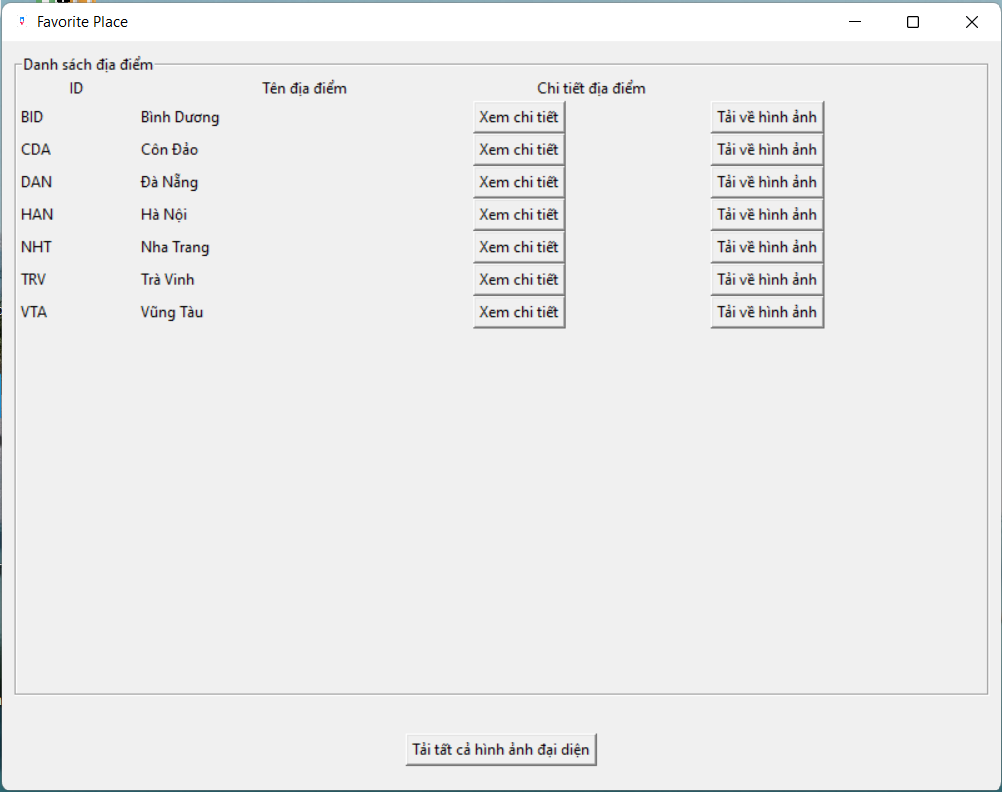
\includegraphics[scale=0.75]{app-description/app}}
\caption{Giao diện phần mềm phía \texttt{client}}
\end{figure}

\large\item \bf Tính năng
\normalsize
\begin{enumerate}
\item \textit{Truy vấn chi tiết thông tin địa điểm}


\item \textit{Tải về tất cả hình ảnh của địa điểm}
\end{enumerate}
\end{enumerate}


\section{Kịch bản giao tiếp của chương trình}
\printbibliography[title = Tài liệu tham khảo]
\end{document}